
% -*- TeX-master: "../dipole_ilya_paper.tex" -*-
\section{Operations with qubits}
\label{sec:characterisation}

% \red{Need scattering data}

\noindent We  record the  energy spectrum  of the twin  qubit while  sweeping the
biasing magnetic  flux.  Because  of a  small asymmetry,  $\eta$, the  fluxes linked
through the left and right loops are $ \Phi = \frac{\varphi}{2\pi}\Phi_0$ and $ \eta\Phi $.

The  \iket{1}~\ilra~\iket{2}  transition,  $\omega_{21}$,  is mapped  with  a  network
analyzer, which measures  the transmission of signal  $\omega_{\text{NA}}$ through the
system.  For  the most part,  the signal  passes through without  any interaction
with  the   qubit  and  after   correcting  for  line  losses,   transmission  is
$  \sim 100\%  $.   Only  near resonance  ($\omega_{\text{NA}}=\omega_{21}$),  does the  qubit
exchange photons  with the  driving field  as it evolves  between the  ground and
excited  states \cite{rabi}.   This evolution  emits a  wave that  is exactly  in
anti-phase  with the  driving field  \cite{abdumalikov2010}, and  the destructive
superposition  in   the  output   line  results  in   a  transmission   dip,  see
Fig.~\ref{fig:transmission}.  The bottom of this dip is plotted with blue circles
for  different points  in the  magnetic flux  to get  the transition  spectrum of
$\omega_{21}$, see inset of Fig.~\ref{fig:transmission}.

\begin{figure}[h]
  \centering 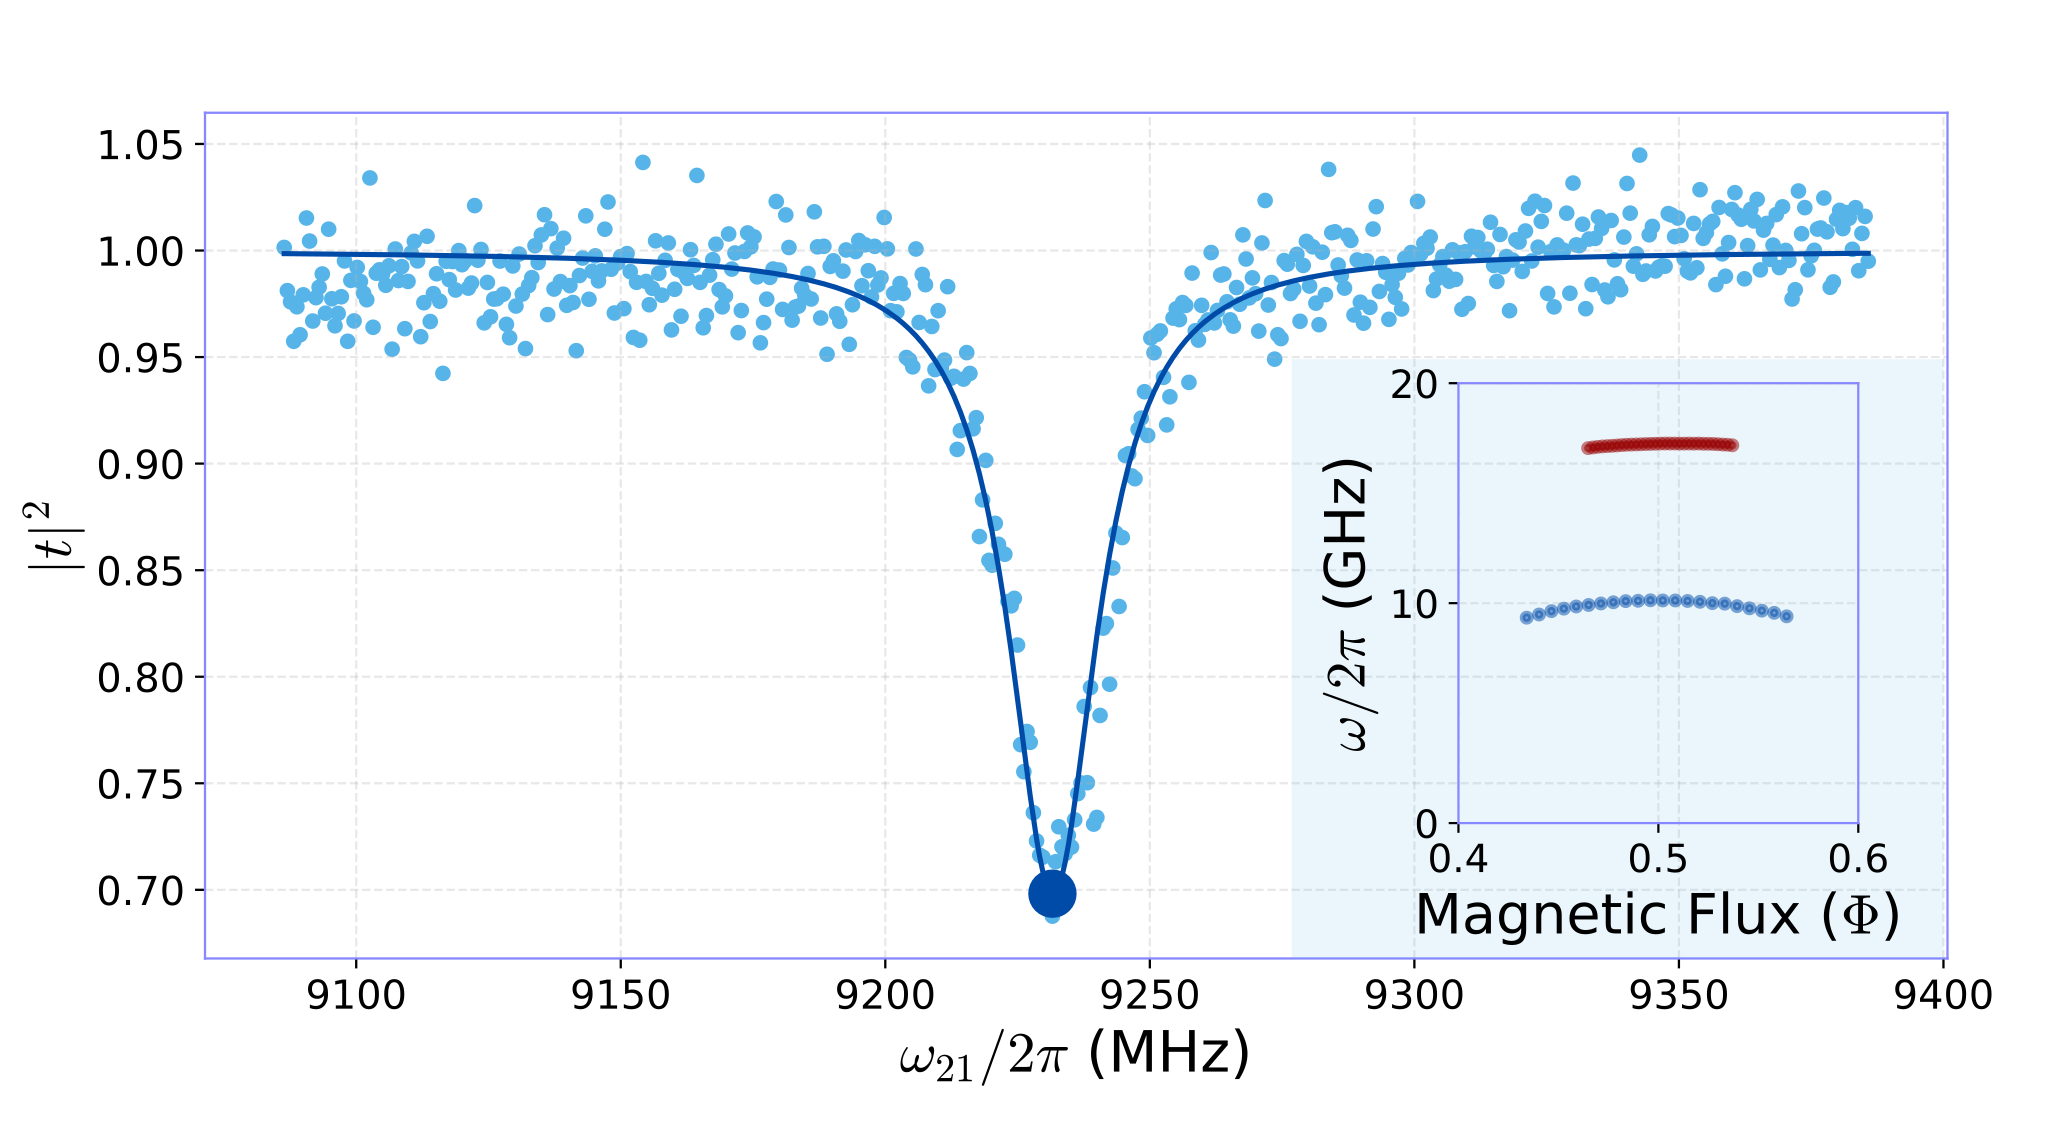
\includegraphics[height = 4.8cm]{fig2.png}
  \caption{\small \textbf{Mapping the qubit  transition spectrum.}  For the lower
    transition  $\omega_{21}$ (blue,  inset)  a network  analyzer  measures the  power
    transmission coefficient, \iabsSquared{t},  at flux bias $ \Phi  $ and microwave
    frequency  $  \omega_{21}/2\pi$.   A   Lorentzian  fit  \cite{Astafiev2010}  to  the
    transmission profile establishes the resonant frequency, which is marked with
    blue points  on the flux-frequency  spectrum.  For transition  $\omega_{32}$ (red,
    inset)  a  two-tone measurement  is  run  by  monitoring  changes to  a  weak
    $\omega_{21}$ probe  while sweeping  a second  frequency in  search of  the higher
    transition.   Any  changes to  the  probe's  transmission are  indicative  of
    hitting  the higher  transition, which  is  marked with  a red  point on  the
    spectrum.     Readings    are    taken    about    the    degeneracy    point
    $ \Phi \sim \Phi_{0}/2  $, where the low curvature of  transition energies, allows for
    stable measurements with respect to fluctuations in the field.}
  \label{fig:transmission}
\end{figure}

The  \iket{2}\ilra\iket{3}   transition,  $\omega_{32}$,  is  mapped   using  two-tone
spectroscopy.   The  network  analyzer  is  tuned  to  the  transition  frequency
$ \omega_{21} $, found  with the first measurement and called  the probe signal, while
an additional generator sweeps a  second frequency, $ \omega_{\text{GEN}} $.  Whenever
the      generator      strikes     the      \iket{2}\ira\iket{3}      transition
($\omega_{\text{GEN}} = \omega_{32} $), the qubit  will be undergo a ladder of excitations,
\iket{1}  \iratext{$\omega_{21}$}\iket{2}  \iratext{$\omega_{32}$}  \iket{3},  depopulating
states \iket{1}  and \iket{2}.   Because of this  depopulation, the  probe signal
becomes less involved with driving and it's  transmission moves out of the dip in
Fig.~\ref{fig:transmission}.  This  identifies $\omega_{32}$ which is  mapped with red
circles.

% prove that state  1 becomes depopulated by solving the  master equation for two
% drives


\begin{figure}[h]
  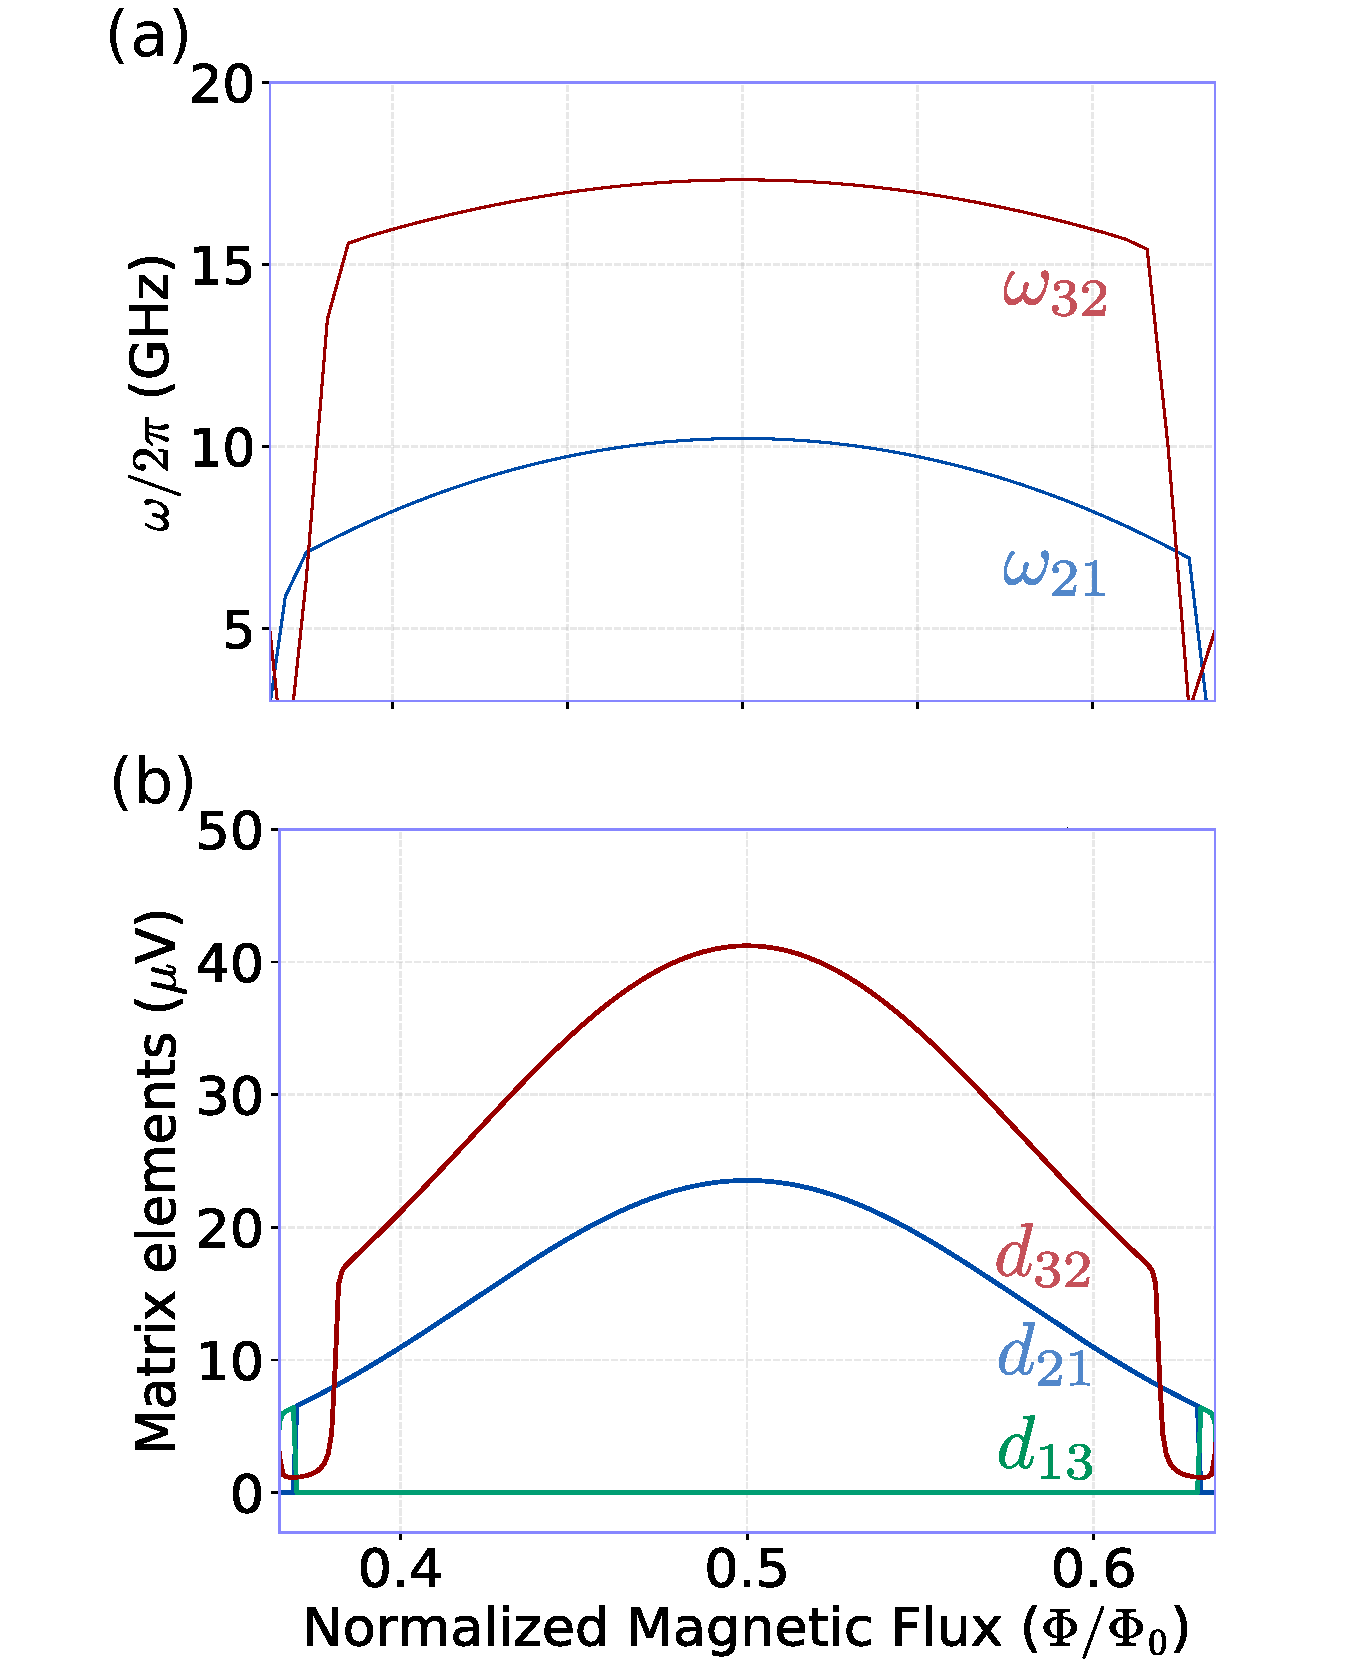
\includegraphics[height=4.7cm]{fig3}
  \caption{\small Transition  frequencies between levels  \iket{1}\ilra \iket{2},
    $ \omega_{21}  $ (blue), and  \iket{2} \ilra \iket{3}, $  \omega_{32}$ (red).
    Readings for  $ \omega_{32} $  are in a narrow  flux range because  away from
    $ \Phi  = (n + \frac{1}{2})\Phi_0,  n\in\mathbb{Z} $, it gets  harder to tune
    the VNA to  $ \omega_{21} $ (as part of  the two-tone spectroscopy procedure)
    which prevents the accurate mapping of  $ \omega_{32} $ with the second tone.
    Asymmetry in  the flux penetrating  the left and  right loops results  in the
    gradual change  of transition frequencies  with every  $ \Phi_{0} $  period -
    $\omega_{21}$ creeps up, while $\omega_{32}$  creeps down, breaking the usual
    spectrum periodicity of flux qubits.}
  \label{fig:experiment}
\end{figure}

We  match the  experimental  data  points to  simulations  made  on the  system's
Hamiltonian, $ \mathcal{H} =  T + U $, developed using  the standard approach for
quantum  electrodynamics  \cite{orlando1999}.  Islands,  isolated  by  the JJ  in
Fig.~\ref{fig:setup},   are   labeled   with    Cooper   pair   (CP)   occupation
$       \vec{n}      =       \iket{n_1,       n_2,       n_3}      $,       phase
$     \vec{\varphi}      =     \iket{\varphi_1,      \varphi_2,     \varphi_3}     $      and     voltage
$ \vec{V} =  \iket{V_{1}, V_{2}, V_{3}} $ states.  An  inspection of the system's
capacitor system links the charges and voltages

\begin{equation}
  \label{eq:link}
  2e\vec{n} = \hat{C}\vec{V}
\end{equation}

\noindent through the capacitance matrix

\begin{equation}
  \label{eq:capac}
  C = \iabs{C} \begin{pmatrix}
    2  &  -1  &  0\\
    -1  &  2  +  \alpha  &  -1\\
    0  &  -1  & 2
  \end{pmatrix},
\end{equation}

\noindent  where \iabs{C}  is the  capacitance of  the outer  JJs.  The  charging
energy,    resulting    from    the     interaction    between    charged    CPs,
$ \vec{Q}=2e\vec{n}  $, and voltages  on the islands,  gives rise to  the kinetic
term of the Hamiltonian:

\begin{equation}\label{eq:kinetic}
  \begin{aligned}
    T = \frac{1}{2}\sum_{i=1}^{3}Q_iV_i & =
    \frac{(2e)^2}{2}\vec{n}\hat{C}^{-1}\vec{n}^{T}\\
    & =  E_C \iabs{C}  \ibra{n_{1}, n_{2},  n_{3}}{\hat{C}^{-1}}\iket{n_{1}, n_2,
      n_3},
  \end{aligned}
\end{equation}

\noindent defining 

Each JJ with a  phase difference of $\Delta\varphi_{i}$ across it,  contributes an energy of
$  E_{Ji}\left(1  -  \cos(\Delta\varphi_i)\right)  $   to  the  potential  term.   The  flux
quantization     condition     for     the      left     and     right     loops,
$ \sum_{i}^{\text{loop}}  \varphi_i = 2\pi n,  n \in \mathbb{Z}$, which  have external biasing
fluxes $ \varphi_\text{ext} $, $ \eta\varphi_\text{ext} $,  enters as a dependence on two of the
junctions:
\begin{equation}\label{eq:potential}
  \begin{aligned}
    U & = E_J\big[4 + \alpha - \alpha\cos(\varphi_{2}) -\cos(\varphi_{1}) -\cos(\varphi_{3}) - \\
    &  \qquad   \cos(\varphi_{2}  -  \varphi_{1}  -   \varphi_{\text{ext}})  -  \cos(\varphi_{2}  -   \varphi_{3}  +
    \eta\varphi_{\text{ext}})\big].
  \end{aligned}
\end{equation}

The  Hamiltonian  is solved  in  the  CP basis,  $\vec{n}  $,  where it's  matrix
representation takes the form

\begin{equation}
  \label{eq:matrix}
  \kbordermatrix{
    & \cdots & \ket{0,0,1} & \ket{0,0,2} & \ket{0,0,3} & \cdots \\
    \vdots & \ddots & \vdots &  \vdots & \vdots & \iddots \\
    \bra{0,0,1} & \cdots & 0 & 0 & 0 & \cdots \\
    \bra{0,0,2} & \cdots & 0 & 0 & 0 & \cdots \\
    \bra{0,0,3} & \cdots & 0 & 0 & 0 & \cdots \\
    \vdots & \iddots & \vdots & \vdots &  \vdots & \ddots
  },
\end{equation}

\noindent

in which the kinetic terms naturally fall on the diagonal and the potential terms
are distributed symmetrically on the off diagonal positions.  The phase operators
in         the          number         basis          representation         read
$   e^{\pm  i\hat{\varphi}_j}   =  \sum_{n_i}\iketbra{n_i\pm1}{n_i}$   \cite{phase}.   The
eigenenergies of  the resulting  Hamiltonian are  compared with  the experimental
data  in Fig.~\ref{fig:experiment}  using \iunit{E_J  = 91.0}{GHz},  \iunit{E_C =
  13.50}{GHz}, \iunit{\alpha  = 1.023}{}, \iunit{\eta  = 1.011}{}.  The  asymmetry value,
$ \eta $, is close the visual loop area difference of 3\% seen from the SEM image in
Fig.~\ref{fig:setup}.

The resonance  is period in  flux, with a tendency  of higher $\omega_{21}$  at higher
magnetic flux numbers.
 
 \begin{figure}[h!]
   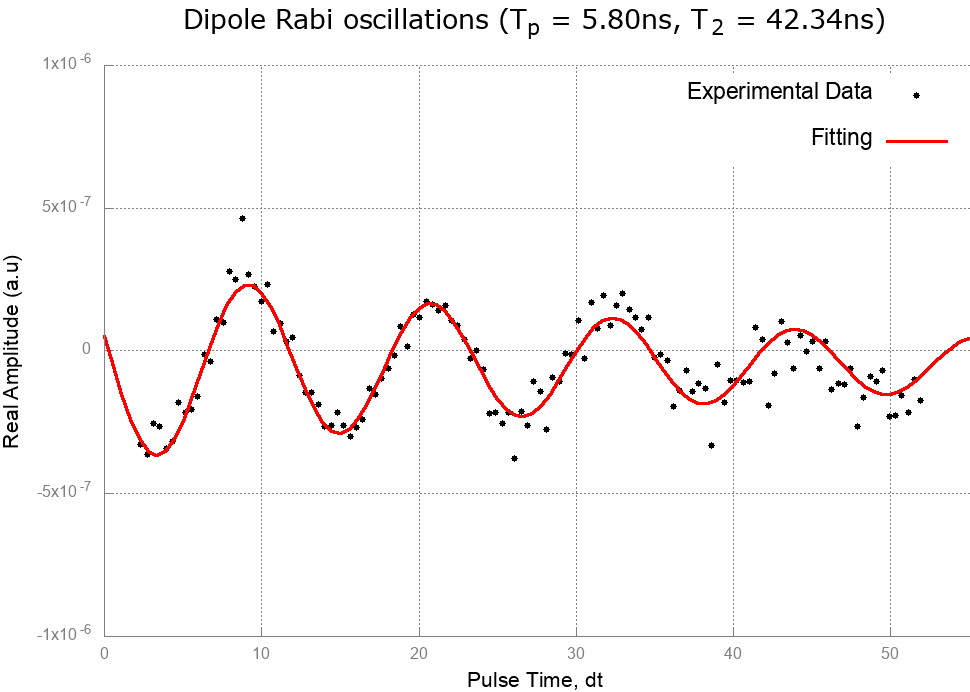
\includegraphics[height = 5cm]{figure5}
   \caption{Rabi oscillation taken at the degeneracy point, $ \Phi_0/2 $, by driving
     the qubit with resonant microwaves,  $\omega_{\text{VNA}} = \omega_{21}$ for different
     time  periods,  $  dt $,  and  monitoring  the  signal  in the  output  line
     \cite{rabi}.         The         a        decoherence         time        of
     $ \tau_{\text{dec}}  = \iunit{42}{ns} $  is extracted from the  decay envelope,
     $ e^{-dt/\tau_\varphi} $, of the the oscillations. \label{fig:rabi}}
 \end{figure}
 An  important qubit  parameter is  the curvature  at the  turning points  in the
 energy spectrum,  where qubit operations  are carried  out.  A low  curvature is
 desirable, to  make the  qubit less  sensitive to  external flux  changes, which
 would  improve  decoherence   time.   At  the  twin   qubits'  degeneracy  point
 $   \Phi   =   (n   +   \frac{1}{2})\Phi_0,   n\in\mathbb{Z}   $,   the   curvature   is
 $   -550\pm10\,\text{GHz}/\Phi_0^2   $.    It   is   substantially   smaller   than
 $  13\times  10^4$ $  \text{GHz}/\Phi_0^2$  on  the  4-JJ flux  qubit  \cite{stern2014},
 $  8.4   \times  10^4$   \cite{zhu2010}  and  $   37\times  10^{4}$   $  \text{GHz}/\Phi_0^2$
 \cite{gustavsson2012}  on  the  3-JJ  flux qubits  demonstrated  recently.   The
 decoherence   time  in   our   qubits  was   however   relatively  small,   only
 $ \tau_\text{dec}  = \iunit{42}{ns}  $.  We get  $\tau_\text{dc}$ from  measurement of
 Rabi  oscillations, see  Fig.~\ref{fig:rabi}  \cite{rabi}.  We  explain this  by
 poisoning of the sample with  infrared radiation, and simplified technology used
 for fabrication as we mentioned above.

 Despite  the twin  qubit have  a much  the decoherence  time in  our qubits  was
 relatively  small  This improved  robustness  to  flux  noise  is matched  by  a
 decoherence time  of , extracted  from Rabi oscillations  in Fig.~\ref{fig:rabi}
 \cite{rabi}.

%%% Local Variables:
%%% mode: latex
%%% TeX-master: "../dipole_ilya_paper"
%%% End:
